\section{Results}
\label{sec:results}

Table~\ref{tab:main} gives every training condition; thresholds are tuned on validation and frozen, and intervals are bootstrapped over diagrams \cite{efron1993bootstrap}.

\begin{table}[tbp]
  \centering\small
  \caption{Macro-F1 against geometric labels at validation-tuned thresholds, seed mean with \ciLevelPct\% bootstrap interval (\nSeedsFt{} seeds; $\dagger$ one seed).}
  \label{tab:main}
  \begin{tabular}{@{}l l l l@{}}
    \toprule
    Training condition & Geometry3K test & PGDP5K held-out & Synthetic extrapolation \\
    \midrule
    Linear probe & \ciProbeId & \ciProbeHo & \ciProbeEx \\
    Fine-tune, real only & \ciFtId & \ciFtHo & \ciFtEx \\
    \quad no highlight$^\dagger$ & \ciNoOverlayId & \ciNoOverlayHo & \ciNoOverlayEx \\
    \quad DINOv2-L backbone$^\dagger$ & \ciDinovId & \ciDinovHo & \ciDinovEx \\
    + 1k synthetic$^\dagger$ & \ciSynOneKId & \ciSynOneKHo & \ciSynOneKEx \\
    + 10k synthetic & \ciSynTenKId & \ciSynTenKHo & \ciSynTenKEx \\
    + 50k synthetic & \ciSynFiftyKId & \ciSynFiftyKHo & \ciSynFiftyKEx \\
    Self-training, confidence & \ciStConfId & \ciStConfHo & \ciStConfEx \\
    Self-training, consistency & \ciStConsId & \ciStConsHo & \ciStConsEx \\
    Control, no pseudo-labels & \ciStControlId & \ciStControlHo & \ciStControlEx \\
    \bottomrule
  \end{tabular}
\end{table}

\paragraph{The eye reads most of it.} A linear head on frozen features reaches \fProbeId{} in distribution and \fProbeHo{} on the unseen source; fine-tuning lifts both to \fFtId{} and \fFtHo{}, the unseen source no worse than the seen one. On the held-out source \hlBothHo\% of queries were solved by the probe already and \hlFinetuneOnlyHo\% only after fine-tuning (Fig.~\ref{fig:headline}); the gain sits in \rel{equal\_length} and \rel{perpendicular} (Fig.~\ref{fig:perrel}). Orientation and incidence were readable from frozen features; comparing two lengths had to be taught.

\begin{figure}[tbp]
  \centering
  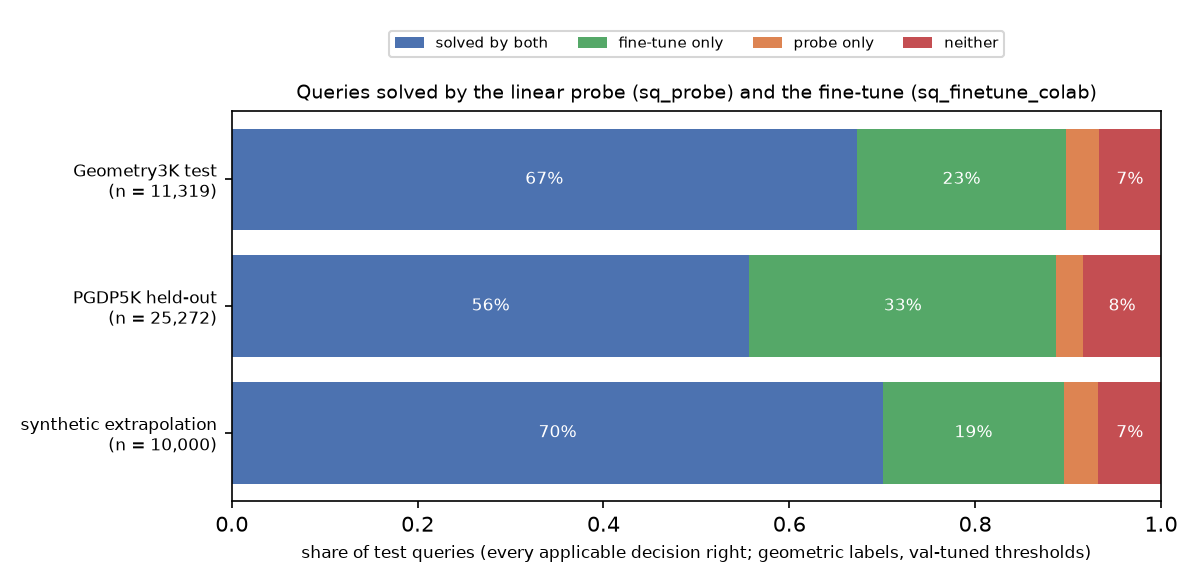
\includegraphics[width=0.95\textwidth]{headline_table}
  \caption{Test queries whose every decision is right under the probe, the fine-tune, both or neither.}
  \label{fig:headline}
\end{figure}

\begin{figure}[tbp]
  \centering
  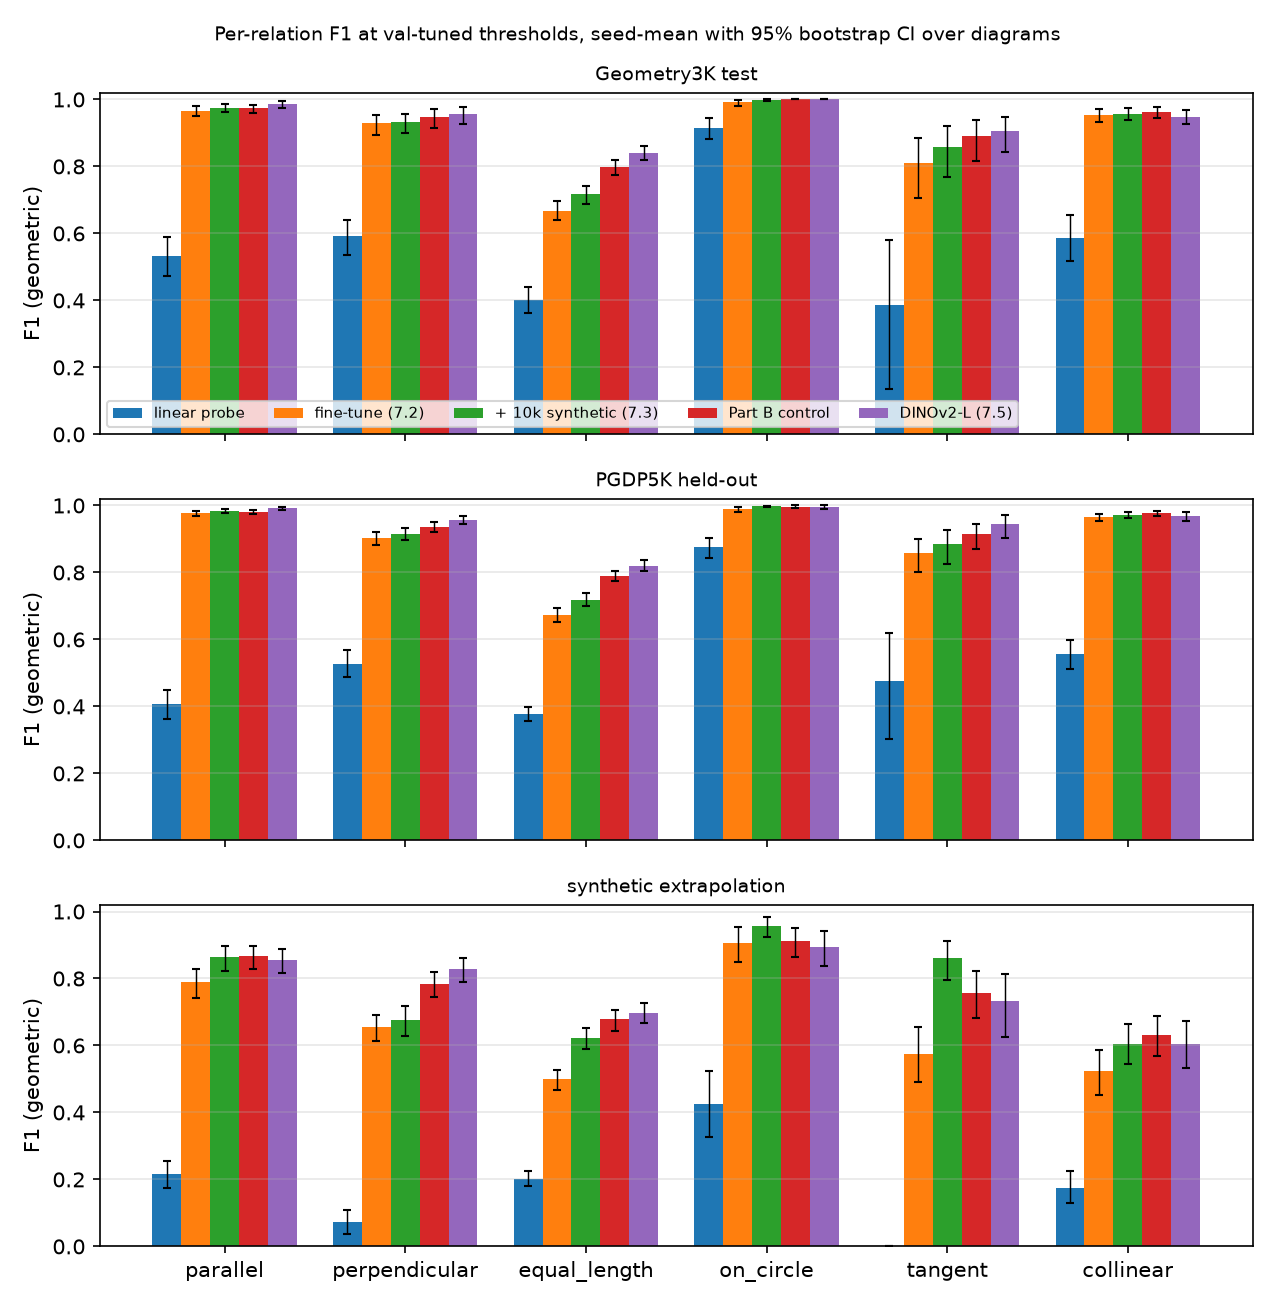
\includegraphics[width=\textwidth]{per_relation_f1}
  \caption{Per-relation F1 with bootstrap intervals.}
  \label{fig:perrel}
\end{figure}

\paragraph{The highlight is the task.} Replacing the overlay by point-name tokens drops macro-F1 to \fNoOverlayId{}, below the frozen probe. The fine-tuned model looks where the highlight is: \attHighlightPct\% of last-layer CLS attention over patch tokens falls on the \attHighlightAreaPct\% of patches the overlay touches (Fig.~\ref{fig:attention}), for wrong decisions as much as right ones, so the errors are not cases of looking elsewhere; attention rollout \cite{abnar2020rollout} is diffuse and kept as a secondary view.

\begin{figure}[tbp]
  \centering
  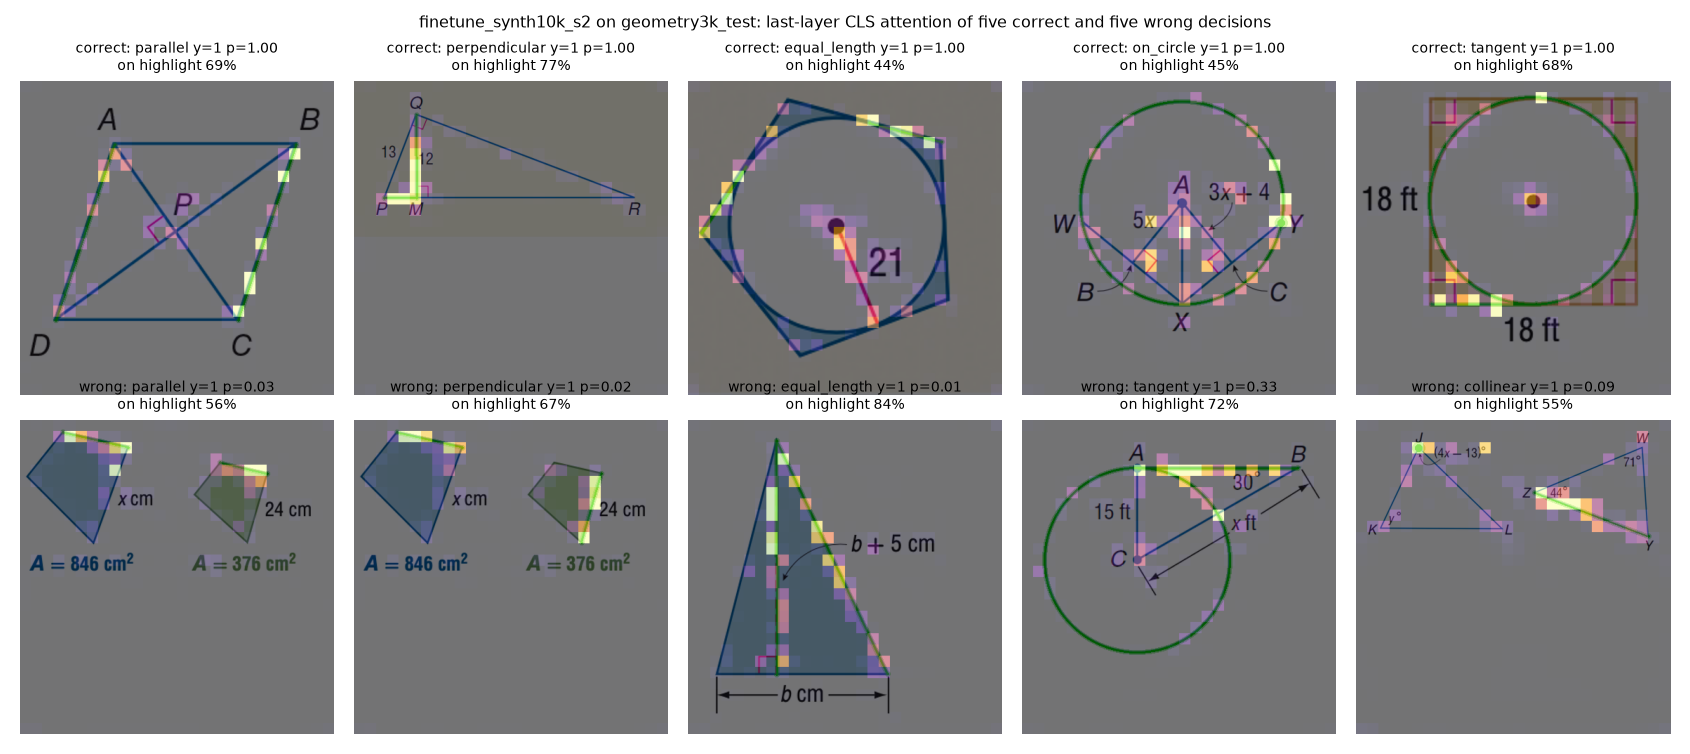
\includegraphics[width=\textwidth]{attention_grid}
  \caption{Last-layer CLS attention for five correct (top) and five confidently wrong (bottom) decisions.}
  \label{fig:attention}
\end{figure}

\paragraph{Where eye and ruler part company.} Fig.~\ref{fig:margin} plots correct decisions against the verifier margin in units of the tolerance. For \rel{parallel} the share falls from \accParallelIdA{} well inside the tolerance to \accParallelIdC{} just inside and \accParallelIdD{} just outside: there the ruler is the poor judge. \rel{equal\_length} is worse in a different way: clear positives are read correctly only \accEqualLengthIdA{} of the time and the dip spans half to twice the tolerance; a \tolEqualLengthPct\% difference in length is below what this eye measures. Size is the second factor: when the shortest queried segment is under a tenth of the diagonal, macro-F1 falls to \fSegShortId{} and \fSegShortHo{} against \fSegLongestId{} and \fSegLongestHo{} for long ones, and \rel{collinear} collapses on short lines, where its tolerance is a few pixels.

\begin{figure}[tbp]
  \centering
  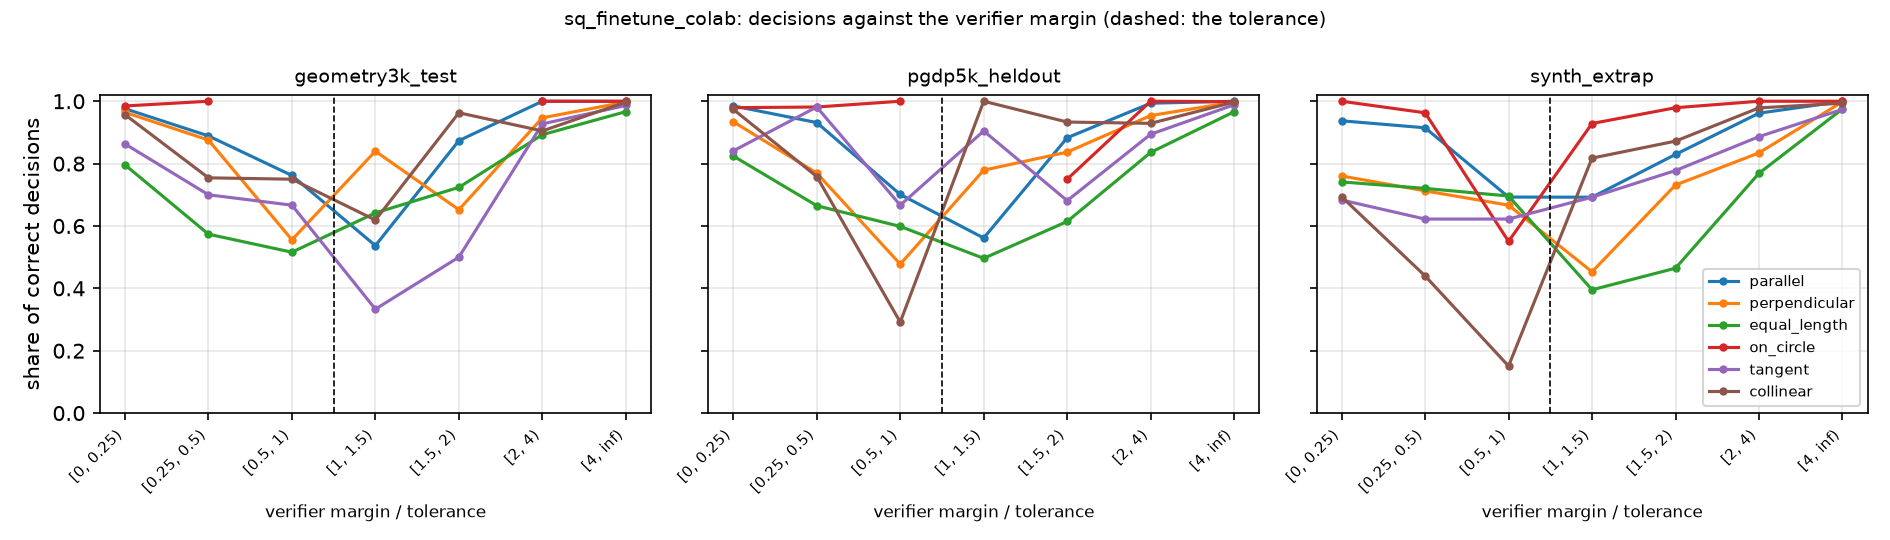
\includegraphics[width=\textwidth]{error_margin}
  \caption{Correct decisions against the verifier margin in units of the tolerance (dashed).}
  \label{fig:margin}
\end{figure}

\paragraph{Part A: the verifier as labeller.} Synthetic diagrams at equal budget leave the in-distribution score flat and move the other two sets (Fig.~\ref{fig:scaling}): the unseen source gains \gainSynTenKHo{} and the extrapolation set \gainSynTenKEx{} with ten thousand diagrams. One thousand already gives \gainSynOneKEx{} there and fifty thousand adds nothing: at this budget, diversity beyond a thousand diagrams is not what the model lacks. Of the one-seed ablations, 224 px costs \gainResId{} in distribution, augmentation changes nothing (\gainAugEx{} on extrapolation), and DINOv2-L under the identical recipe gains \gainDinovId{}, more than any data intervention, which with one seed we record rather than explain.

\begin{figure}[tbp]
  \centering
  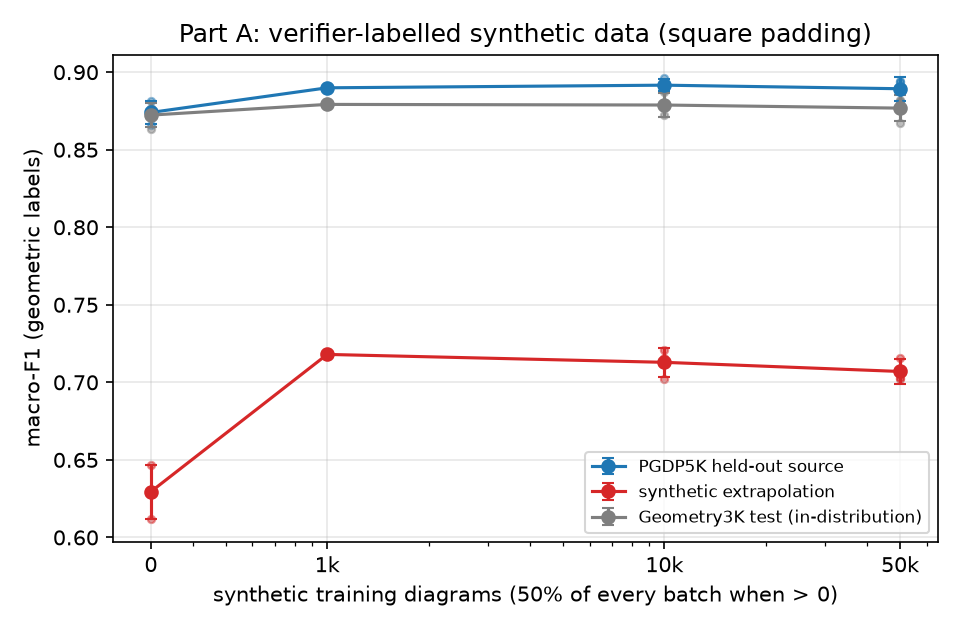
\includegraphics[width=0.78\textwidth]{scaling_square}
  \caption{Macro-F1 against synthetic training diagrams at a fixed budget.}
  \label{fig:scaling}
\end{figure}

\paragraph{Part B: self-training did not pay.} We pseudo-labelled \stPoolDiagrams{} PGPS9K diagrams with the 10k-synthetic model \cite{xie2020noisystudent} above confidence \selftrainTau{}, with and without a deductive filter that drops any diagram whose predicted relations contradict each other after closure. The filter raised pseudo-positive precision from \stPrecisionConf{} to \stPrecisionCons{}. Then the control, the same continued training with no pseudo-labels, beat both students: \fStControlHo{} against \fStConsHo{} and \fStConfHo{} on the held-out source. The pseudo-labels, half of every batch, cost about what the filter recovered. I read this as a budget result rather than a verdict on the filter: \rel{equal\_length} pseudo-labels were only \stPrecisionConfEqualLength{} precise, and that is where the students lost ground. Every checkpoint was re-evaluated with each query padded alone, because batch padding had let a decision depend on its neighbours; the appendix gives the effect, which changed no conclusion.
